\documentclass[a4paper,12pt,final]{article}
% Pour une impression recto verso, utilisez plutôt ce documentclass :
%\documentclass[a4paper,11pt,twoside,final]{article}

\usepackage[english,francais]{babel}
\usepackage[utf8]{inputenc}
\usepackage[T1]{fontenc}
\usepackage[pdftex]{graphicx}
\usepackage{setspace}
\usepackage{hyperref}
\usepackage[french]{varioref}
\usepackage[top=3cm, bottom=2.8cm, left=2cm, right=2cm]{geometry}
%\usepackage{a4wide}
 \usepackage{textcomp}
\usepackage{amsmath}
\usepackage{listings}
\usepackage{color}

\definecolor{mygreen}{rgb}{0,0.6,0}
\definecolor{mygray}{rgb}{0.5,0.5,0.5}
\definecolor{mymauve}{rgb}{0.58,0,0.82}

\lstset{ %
  backgroundcolor=\color{white},   % choose the background color; you must add \usepackage{color} or \usepackage{xcolor}
  %basicstyle=\footnotesize,        % the size of the fonts that are used for the code
  breakatwhitespace=true,         % sets if automatic breaks should only happen at whitespace
  breaklines=false,                 % sets automatic line breaking
  captionpos=b,                    % sets the caption-position to bottom
  commentstyle=\color{mygreen},    % comment style
  extendedchars=true,              % lets you use non-ASCII characters; for 8-bits encodings only, does not work with UTF-8
  frame=single,                    % adds a frame around the code
  keepspaces=false,                 % keeps spaces in text, useful for keeping indentation of code (possibly needs columns=flexible)
  keywordstyle=\color{blue},       % keyword style
  language=SQL,                 % the language of the code
  morekeywords={*,...},            % if you want to add more keywords to the set
  numbers=none,                    % where to put the line-numbers; possible values are (none, left, right)
  numbersep=5pt,                   % how far the line-numbers are from the code
  numberstyle=\tiny\color{mygray}, % the style that is used for the line-numbers
  rulecolor=\color{black},         % if not set, the frame-color may be changed on line-breaks within not-black text (e.g. comments (green here))
  stringstyle=\color{mymauve},     % string literal style
  tabsize=2,                       % sets default tabsize to 2 spaces
}

\lstset{literate=
  {á}{{\'a}}1 {é}{{\'e}}1 {í}{{\'i}}1 {ó}{{\'o}}1 {ú}{{\'u}}1
  {Á}{{\'A}}1 {É}{{\'E}}1 {Í}{{\'I}}1 {Ó}{{\'O}}1 {Ú}{{\'U}}1
  {à}{{\`a}}1 {è}{{\`e}}1 {ì}{{\`i}}1 {ò}{{\`o}}1 {ù}{{\`u}}1
  {À}{{\`A}}1 {È}{{\'E}}1 {Ì}{{\`I}}1 {Ò}{{\`O}}1 {Ù}{{\`U}}1
  {ä}{{\"a}}1 {ë}{{\"e}}1 {ï}{{\"i}}1 {ö}{{\"o}}1 {ü}{{\"u}}1
  {Ä}{{\"A}}1 {Ë}{{\"E}}1 {Ï}{{\"I}}1 {Ö}{{\"O}}1 {Ü}{{\"U}}1
  {â}{{\^a}}1 {ê}{{\^e}}1 {î}{{\^i}}1 {ô}{{\^o}}1 {û}{{\^u}}1
  {Â}{{\^A}}1 {Ê}{{\^E}}1 {Î}{{\^I}}1 {Ô}{{\^O}}1 {Û}{{\^U}}1
  {œ}{{\oe}}1 {Œ}{{\OE}}1 {æ}{{\ae}}1 {Æ}{{\AE}}1 {ß}{{\ss}}1
  {ç}{{\c c}}1 {Ç}{{\c C}}1 {ø}{{\o}}1 {å}{{\r a}}1 {Å}{{\r A}}1
  {€}{{\EUR}}1 {£}{{\pounds}}1
}


\usepackage[final]{pdfpages}
\makeatletter
\renewcommand%
{\subsection}{\@startsection{subsection}{2}{10mm}
{-\baselineskip}{0.25\baselineskip}%
{\bf\large\slshape}}%
\makeatother

\makeatletter
\renewcommand%
{\subsubsection}{\@startsection{subsubsection}{2}{20mm}
{-\baselineskip}{0.25\baselineskip}%
{\normalfont\large\slshape}}%normalsize
\makeatother

\newcommand{\reporttitle}{Lab 1 : Intelligent Agents}     % Titre
\newcommand{\reportauthor}{Daniel \textsc{Robox} Fanjie\textsc{Nie}} % Auteur
\newcommand{\reportsubject}{TDDC17 Artificial Intelligence} % Sujet
\newcommand{\HRule}{\rule{\linewidth}{0.5mm}}
\setlength{\parskip}{1ex} % Espace entre les paragraphes

\hypersetup{
    pdftitle={\reporttitle},%
    pdfauthor={\reportauthor},%
    pdfsubject={\reportsubject},%
    pdfkeywords= {lab1, agents, intelligent}
}

\begin{document}
  \begin{titlepage}
\thispagestyle{empty}
\begin{center}

\begin{minipage}[t]{0.48\textwidth}
  \begin{flushleft}
    
\includegraphics [width=48mm]{images/logo-univ.jpg} \\[0.5cm]

  \end{flushleft}
\end{minipage}
\begin{minipage}[t]{0.48\textwidth}
  \begin{flushright}

  \end{flushright}
\end{minipage} \\[1.0cm] %1.5

\vspace{5.3cm}

\textsc{\Large \reportsubject :}\\[2cm]

\HRule \\[0.4cm]
{\Large \bfseries \reporttitle}\\[0.4cm]
\HRule \\[1.5cm]

\vspace{1.5cm}

%\includegraphics [width=80mm]{images/ascii_art2.png} \\[0.5cm]
\vspace{4cm}
\begin{minipage}[t]{0.30\textwidth}
  \begin{flushleft} \normalsize
     ~Daniel \textsc{Roxbo}\\
	 ~Fanjie \textsc{Nie} \\                
 \end{flushleft}
\end{minipage}
\begin{minipage}[t]{0.6\textwidth}
  \begin{flushright} \normalsize

    %~Daniel \textsc{Roxbo} \\
	%~Fanjie \textsc{Nie} \\
  \end{flushright}
\end{minipage}

\vfill
\vspace*{0.420cm}
{\large September 2016 }

\end{center}
\end{titlepage}

  \cleardoublepage
  %\section*{Introduction} % Pas de numérotation
\addcontentsline{toc}{section}{Introduction} % Ajout dans la table des matières
    \thispagestyle{empty}
 \setcounter{page}{1}
\vspace{2cm}

  %\tableofcontents
  %\sloppy
  %\cleardoublepage
  \cleardoublepage
  %section{Analyse du sujet et structure du projet}
 %\setcounter{page}{2}
 \addtocounter{section}{0}
 \thispagestyle{empty}
\section{Task1}
The agent must be able to suck up all dirt in a rectangular world of unknown dimensions without obstacles and shut down on the home position (home position can be sensed through one of the percepts). At the end the agent should also have a fully updated world model (i.e. world variable in MyAgentState class). 

\subsection{Decision-Loop}
The first assignement does not imply obstacle avoidance, it is possible
to implement an easy 3-step strategy :

\begin{itemize}
  \item First, move the VacuumAgent back to its home position, (1,1) on the grid, after it has performed its initial random moves.
  \item Moving forward horizontaly and once we hit a wall we move one step south and continue in the opposite direction.
  \item Finally when the VacuumAgent turns 90° to south and bump into the south wall, it goes back to the home position.
\end{itemize}

\subsection{Possible improvement}

The VacuumAgent have the ability to suck up all dirt in a rectangular world of unknown dimensions without obstacles and shut down on the home position in this way.But the world model can't be fully updated at the end.There is still (?) in the map where some of the wall is.This problem will be solved in task2.

\section{Task2}
Extend and improve your agent to be able to solve the problem with obstacles (0.1 obstacle density, 15x15 world).

\subsection{Decision-Loop}
Our agent is searching for all the unknown squares that we have access to, directly or indirectly. The search is performed with a slightly modified version of the Uniform-Cost Search, where the only significant difference is that we do not replace the elements in the frontier with possibly cheaper elements. When an unknown square is found we move over there using the path acquired by the search method.

\subsection{Data stored in Agent}
Search is containing all the logic related to finding a cheap path to a certain square type.We combine Actions into Moves, and Moves into objects called Paths to simplify the logic. This enables us to think of the problem at a higher level.
\begin{itemize}
	\item \textbf{actionSequence}
When we have found a suitable path we store all of its actions in the actionSequence container which is a queue.
	\item \textbf{frontier}
Is a PriorityQueue containing paths, and is sorted on the lowest path cost. The cost consists of the number of actions required to execute the path.
	\item \textbf{Explored}
Contains the string representation of the coordinates for explored squares.
\end{itemize}
\subsection{Reasons we choose the solusions }
We could not come up with any simple rules that would solve the problem of avoiding/moving around obstacles. Especially difficult would be differentiating between random obstacles and the wall. Our search based solution will always explore 100\% of accessible map in 100\% of runs.

\begin{figure}[h]
    \centering
      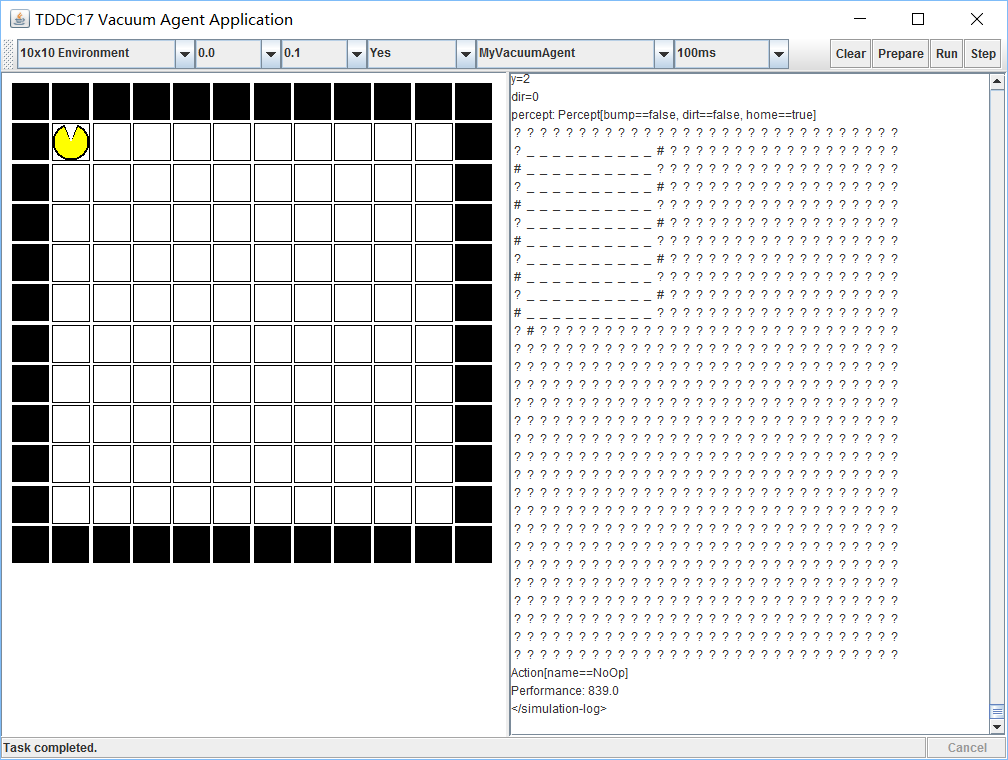
\includegraphics[width=0.83\linewidth]{./images/task1.png}
    \caption{Task1 Screenshot\label{VacuumAgent}}
\end{figure}


\begin{figure}[h]
    \centering
      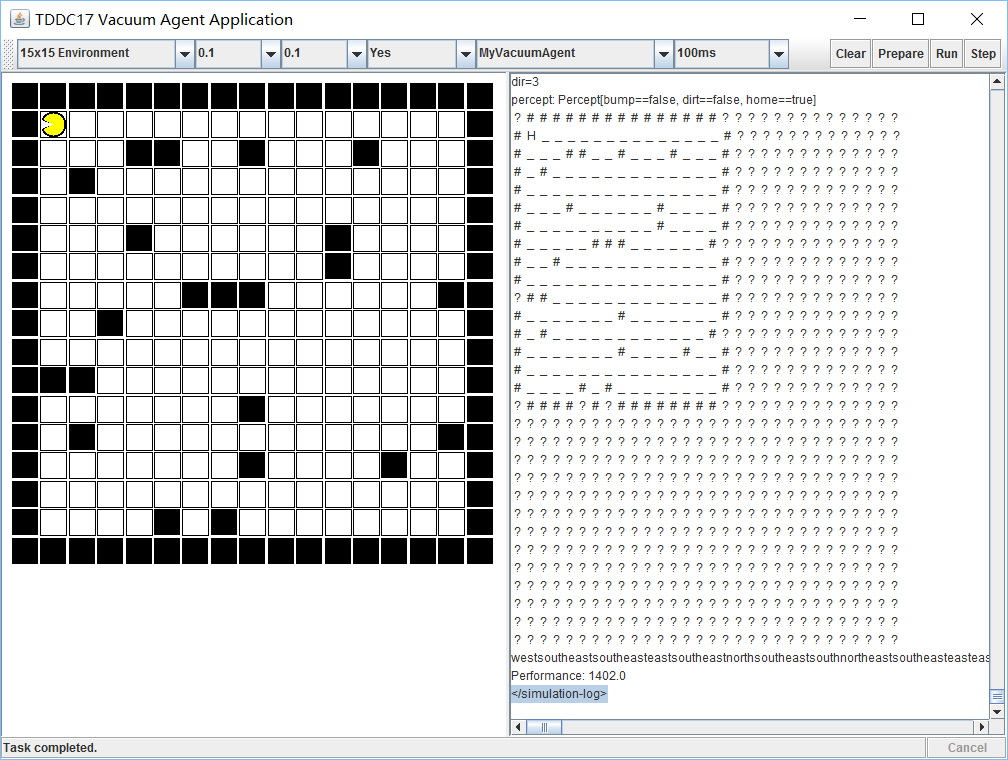
\includegraphics[width=0.83\linewidth]{./images/task2.png}
    \caption{Task2 Screenshot\label{VacuumAgent}}
\end{figure}
\thispagestyle{empty}


  \cleardoublepage
  %\include{partie2}
  %\cleardoublepage
  %\include{partie3}
  %\cleardoublepage
  %\section*{Conclusion}
\addcontentsline{toc}{section}{Conclusion}
\vspace{2cm}

  %\cleardoublepage
\end{document}
